 \section{Durchführung}
\label{sec:Durchführung}


\subsection{Aufbau}

Für die Messreihen 1. und 2. werden für die Kondensatoren und Spulen die
Bauteile mit

\begin{align}
  C_1 & = \SI{20}{\nano\F} & C_2 & = \SI{10}{\nano\F} \\
  L & = \SI{1.217}{\milli\henry}
\end{align}
verwendet. Für die restlichen Messreihen werden für die Kondensatoren und Spulen
Bauteile mit

\begin{align}
  C_1 & = \SI{22}{\nano\F} & C_2 & = \SI{9.39}{\nano\F} \\
  L & = \SI{1.75}{\milli\henry}
\end{align}
verwendet.
Da die Anzeigeskala an dem verwendeten Frequenzgenerator nicht verlässlich ist,
wird in jeder Schaltung ein Frequenzmessgerät mit dem Generator parallel
geschaltet.
In Abbildung \ref{fig:DK} ist die Schaltung zur Aufnahme der Durchlasskurve,
also der Ausgangsamplitude in Abhängigkeit von der Frequenz abgebildet.
Diese Schaltung wird in Messung 1. für die normale und
alternierende LC-Kette benötigt und in der 3. bis 5. Messung in abgewandelter
Form.

\begin{figure}
  \centering
  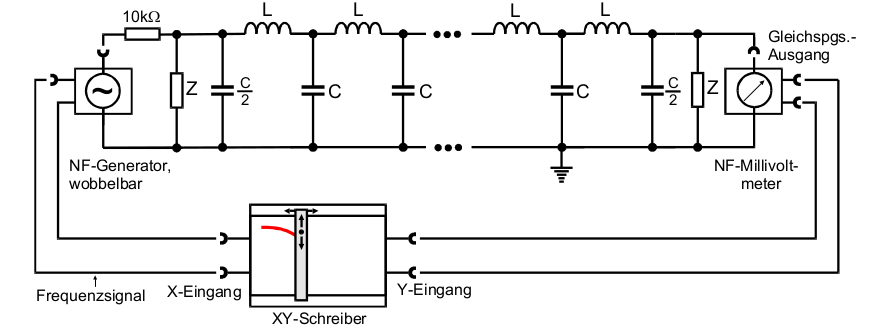
\includegraphics[height=3cm]{DurchlasskurveLCkette.png}
  \caption{Schaltung zur Aufnahme der Durchlasskurve \cite{anleitung}.}
  \label{fig:DK}
\end{figure}

In Abbildung \ref{fig:DR} ist die Schaltung zur Messung der Dispersionsrelation
dargestellt. Diese Schaltung wird in Messung 2. für die normale und die
alternierende LC-Kette benötigt.

\begin{figure}
  \centering
  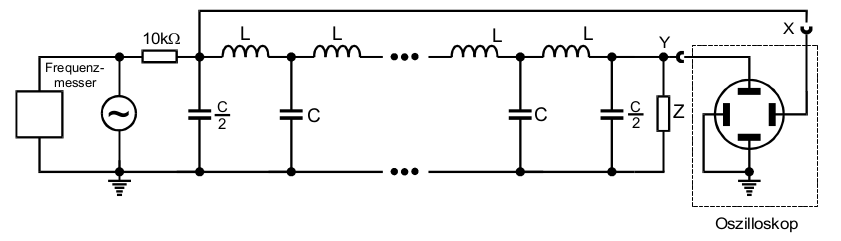
\includegraphics[height=3cm]{DispersionC1C2.png}
  \caption{Schaltung zur Aufnahme der Dispersionsrelation\cite{anleitung}.}
  \label{fig:DR}
\end{figure}


\subsection{Messablauf}

\begin{enumerate}

\item
Bei der ersten Messreihe wird zunächst die Schaltung in Abbildung
\ref{fig:DK} jeweils für eine LC- und für eine $LC_1C_2$-Kette aufgebaut.
Nun muss
bei abgeschalteten Geräten der Wellenwiderstand, den man mit Hilfe der
Gleichung \eqref{eqn:WaveWiderstand} bestimmen kann, mit Hilfe eines
Widerstandsmessgerätes
an beiden Enden der Kette auf

\begin{equation}
Z = \SI{287.05}{\ohm}
\end{equation}
gestellt werden.
Anschließend wird jeweils ein geeigneter Frequenzbereich bei etwa

\begin{equation}
\omega = \SI{50}{\kilo\Hz}
\end{equation}
gewählt und dort die Durchlasskurve mit Hilfe des
XY-Schreibers aufgezeichnet.

\item
Bei der zweiten Messreihe wird zunächst die Schaltung in Abbildung
\ref{fig:DR} jeweils für eine LC- und für eine $LC_1C_2$-Kette aufgebaut.
Nun werden Frequenzmesswerte bei bestimmten Lissajous-Figuren aufgenommen.
Gesucht sind die Figuren, die bei einer Phasenverschiebung $\theta = k\pi$
entstehen.

\item
Bei der dritten Messreihe wird zunächst wieder die Schaltung in Abbildung
\ref{fig:DK} für eine offene LC-Kette ohne den XY-Schreiber, die
Wobbeleinrichtung und die Wellenwiderstände aufgebaut. Sobald eine
stehende Welle am Kettenanfang oder -ende festgestellt wurde, wird jeweils
die Eigenfrequenz notiert.

\item
Bei der vierten Messreihe wird mit derselbe Schaltung jeweils bei der ersten und
zweiten Eigenschwingung an jedem Kettenglied die Spannung mit einem
Milli-Voltmeter bestimmt.

\item
Bei der letzten Messung wird die Messung 4. mit angeschlossenem Wellenwiderstand
$Z$ am Ende der Kette durchgeführt.

\end{enumerate}
